\documentclass[11pt,a4paper]{article}
\usepackage[margin=2.1cm,top=1.9cm,bottom=2.1cm]{geometry}
\usepackage{amsmath,amssymb,amsthm}
\usepackage{booktabs,array,tabularx}
\usepackage{enumitem}
\usepackage{eurosym}
\usepackage{graphicx}
\usepackage{float}
\usepackage{xcolor}
\usepackage[font=small,labelfont=bf]{caption}
\usepackage[hidelinks]{hyperref}
\usepackage{titlesec}
\titlespacing*{\section}{0pt}{9pt}{4pt}
\titlespacing*{\subsection}{0pt}{6pt}{3pt}
\setlength{\parskip}{3pt}
\setlength{\parindent}{0pt}
\setlist{itemsep=1pt,topsep=2pt}

\newtheorem{proposition}{Proposition}
\newcommand{\Dset}{\mathcal{D}}
\newcommand{\Sset}{\mathcal{S}}
\newcommand{\Oset}{\mathcal{O}}
\newcommand{\Kset}{\mathcal{K}}
\newcommand{\Tset}{\mathcal{T}}
\newcommand{\Gset}{\mathcal{G}}
\newcommand{\soc}{\text{soc}}
\newcommand{\midd}{\text{mid}}
\newcommand{\fre}{\text{free}}
\newcommand{\inv}{\text{inv}}
\newcommand{\cor}{\text{corp}}
\newcommand{\M}[1]{\EUR{#1}\,m}

\begin{document}

{\LARGE\bfseries Designing the residential tower for maximum profit}\\[3pt]
{\large Optimal floor plans for 23, 40 and 56 floors}\\[4pt]
{\small Report for the real estate developer \quad$\cdot$\quad Prepared by: Grace Chang \quad$\cdot$\quad October 2026}

\vspace{-2pt}\noindent\rule{\textwidth}{0.4pt}

\section{Summary}

We determined, for each of the three tower heights under consideration, the
design that maximises your profit while meeting all twelve design restrictions:
which floor design to use on every floor, who buys each floor, and the sector
of every apartment. All three solutions are proven optimal and were checked
apartment by apartment against every restriction.

\begin{center}
\begin{tabular}{@{}lrrr@{}}
\toprule
 & \textbf{23 floors} & \textbf{40 floors} & \textbf{56 floors} \\
\midrule
Maximum profit            & \M{17.5} & \M{29.6} & \M{39.2} \\
Profit per floor          & \EUR{760}k & \EUR{741}k & \EUR{700}k \\
Apartments                & 193 & 334 & 464 \\
\bottomrule
\end{tabular}
\end{center}

\textbf{Key findings.}
\begin{itemize}[leftmargin=*]
\item \textbf{Almost all profit comes from large free-sector apartments sold to
  private buyers.} Every solution places as many 131\,m$^2$ penthouse floors
  (design ee) at the top of the tower as the rules allow; each such floor earns
  \M{1.74}--1.77.
\item \textbf{The rest of the tower exists to make those penthouses allowed.}
  Because at least 40\% social and 40\% middle apartments are required, free
  apartments can be at most 20\% of all apartments. The lower floors are
  therefore filled with many small investor apartments (design aa, 12 per
  floor), which add apartments cheaply and keep the 20\% free quota as large as possible.
\item \textbf{The sector quotas are by far the most expensive rules.} Without
  the 40\% social or 40\% middle requirement, profit would be about one third
  higher. The minimum average size of middle apartments (50\,m$^2$) costs
  another 10--14\%. Six restrictions cost nothing at all.
\item \textbf{A taller tower earns more in total, but less per floor}, because
  the profit per apartment falls as the building gets taller.
\end{itemize}

\section{The design problem}

The tower has a fixed number of floors. For every floor you choose one of 11
pre-approved floor designs (aa, ab, \dots, ee), each consisting of two of five
floor parts with given apartment sizes (36--131\,m$^2$). Every apartment is
assigned to a \emph{sector} (social, middle or free) and sold to a
\emph{buyer} (housing corporation, investor or private buyer). The profit of an
apartment depends on its size, sector, buyer and the tower height; we used the
profit tables you supplied for towers of 69\,m, 120\,m and 168\,m, i.e.\ 23, 40
and 56 floors of 3\,m. The design must satisfy the following restrictions.

\begin{center}\small
\begin{tabularx}{\textwidth}{@{}l X l X@{}}
\toprule
\multicolumn{4}{@{}l}{\emph{Whole tower}}\\
R1 & at least 40\% of apartments social & R3 & social apartments at least 40\,m$^2$ on average\\
R2 & at least 40\% of apartments middle & R4 & middle apartments at least 50\,m$^2$ on average\\
R9 & at least 70\% of apartments sold to investors & & \\
\midrule
\multicolumn{4}{@{}l}{\emph{Individual apartments}}\\
R5 & corporation social apartments $\ge 40$\,m$^2$ & R7 & free apartments $\ge 60$\,m$^2$\\
R6 & corporation middle apartments $\ge 50$\,m$^2$ & R8 & corporations buy no free apartments\\
\midrule
\multicolumn{4}{@{}l}{\emph{Floors}}\\
R10 & one buyer per floor & R11 & no social and free apartments on the same floor\\
R12 & \multicolumn{3}{l}{a floor with a smaller smallest apartment lies lower in the tower}\\
\bottomrule
\end{tabularx}
\end{center}

\section{How we found the best design}

We formulated the problem as a mathematical optimisation model (a mixed-integer
linear program, Appendix~A) and solved it with the open-source solver CBC. Instead of
deciding floor by floor, the model decides \emph{how many} floors of each kind
to build (design, buyer and whether the floor may hold free apartments) and
\emph{how many} apartments of each size go to each sector. The floors are then
stacked in order of their smallest apartment, which satisfies R12 automatically.
This keeps the model small: 143 decision variables and 56 constraints,
whatever the height of the tower. Each case is solved to proven optimality in
under two seconds, so new profit figures or rules can be evaluated instantly.

To make sure the results are correct we (i) converted every solution into an
explicit apartment-by-apartment floor plan and checked all twelve restrictions
and the profit on it, and (ii) compared the optimum with a separate, much
larger model that describes every floor individually, which found the same
maximum profit (Appendix~C).

\section{The optimal designs}

\begin{table}[h]
\centering\small\setlength{\tabcolsep}{5pt}
\begin{tabular}{@{}lrrr@{}}
\toprule
 & \textbf{23 floors} & \textbf{40 floors} & \textbf{56 floors} \\
\midrule
Profit                                   & \M{17.48} & \M{29.62} & \M{39.19} \\
Apartments / floor area & 193 / 11\,822\,m$^2$ & 334 / 20\,568\,m$^2$ & 464 / 28\,794\,m$^2$ \\[2pt]
Social apartments (avg.\ size)           & 78 (40.0\,m$^2$) & 134 (40.0\,m$^2$) & 186 (40.0\,m$^2$) \\
Middle apartments (avg.\ size)           & 78 (50.2\,m$^2$) & 134 (50.0\,m$^2$) & 186 (50.0\,m$^2$) \\
Free apartments (avg.\ size)             & 37 (129\,m$^2$) & 66 (129\,m$^2$) & 92 (131\,m$^2$) \\[2pt]
Investor / private / corp.\ buyers & 150 / 36 / 7 & 262 / 64 / 8 & 358 / 92 / 14 \\
Investor share (rule: $\ge 70\%$)         & 77.7\% & 78.4\% & 77.2\% \\[2pt]
Profit from free / middle / social        & \M{16.0} / 1.4 / 0.1 & \M{28.4} / 1.8 / $-$0.6 & \M{40.0} / 1.1 / $-$1.9 \\[2pt]
Floor designs used                        & aa$\times$11, ac, cc, cd, & aa$\times$16, ab, ac$\times$5, & aa$\times$24, ac$\times$7, \\
                                          & ee$\times$9 & bc, cc, ee$\times$16 & cc, ce, ee$\times$23 \\
\bottomrule
\end{tabular}
\caption{Optimal design for each tower height. Full floor-by-floor plans are in Appendix~B.}
\label{tab:results}
\end{table}

\begin{figure}[h]
\centering
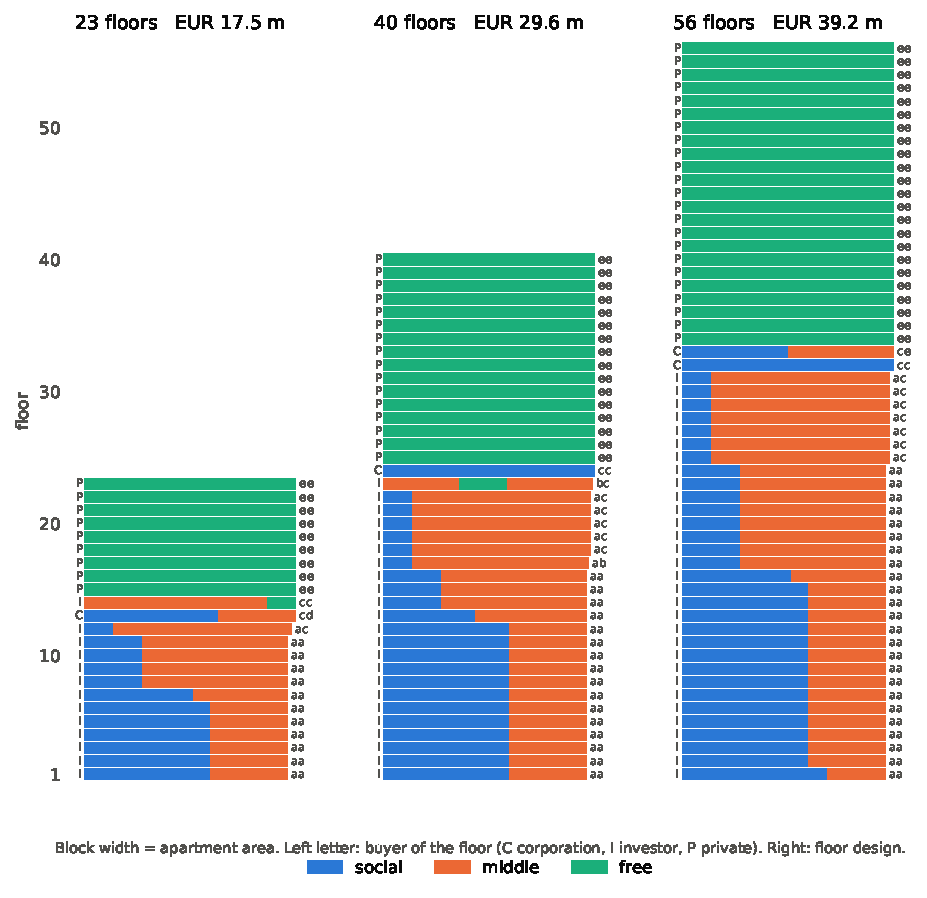
\includegraphics[width=0.93\textwidth]{fig_towers.pdf}
\caption{The three optimal towers. Each row is a floor; each block an apartment.}
\label{fig:towers}
\end{figure}

All three designs follow the same recipe (Figure~\ref{fig:towers}):
\begin{enumerate}[leftmargin=*]
\item \textbf{Top: private penthouse floors.} Design ee (four 131\,m$^2$
  apartments) sold to private buyers in the free sector. One such apartment
  earns about \EUR{435}--444k; no other combination comes close.
\item \textbf{Bottom: small investor apartments.} Design aa (twelve apartments
  of 36--48\,m$^2$) sold to investors as social and middle housing. These
  apartments earn little or even lose money, but each one raises the number of
  free apartments allowed by the 20\% ceiling.
\item \textbf{Middle: a few ``balancing'' floors.} Social apartments must
  average 40\,m$^2$ and middle apartments 50\,m$^2$, while the aa floors are
  smaller. A few floors with larger apartments (ac, cc, cd, ce) lift the
  averages to exactly the minimum. Large social apartments are sold to a
  housing corporation, because for corporations they lose the least money.
\end{enumerate}
In every case the social and middle shares are at (or just above) 40\%
and both average-size limits are met with almost no slack: these rules
determine the design. The investor share (77--78\%) is comfortably above 70\%
without any effort.

\section{Which restrictions cost profit}

To show where the profit is lost, we re-optimised each case with one
restriction removed at a time (Figure~\ref{fig:sens}). The difference is the
cost of that restriction to you.

\begin{figure}[H]
\centering
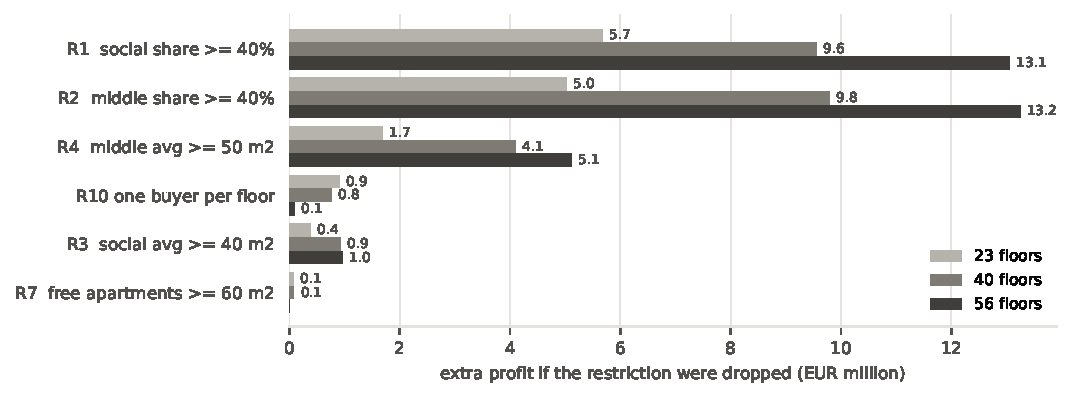
\includegraphics[width=0.85\textwidth]{fig_sensitivity.pdf}
\caption{Extra profit if a single restriction were dropped. Restrictions R5,
R6, R8, R9, R11 and R12 have no cost in any case and are not shown.}
\label{fig:sens}
\end{figure}

\begin{itemize}[leftmargin=*]
\item \textbf{R1 and R2 (40\% social, 40\% middle)} each cost about one third of
  the profit (\M{5.0}--13.2). Any room in these quotas directly turns
  into more penthouses.
\item \textbf{R4 (middle at least 50\,m$^2$ on average)} costs \M{1.7}--5.1
  (10--14\%), because it forces larger, loss-making middle apartments. R3, the
  social counterpart, costs much less (\M{0.4}--1.0).
\item \textbf{R10 (one buyer per floor)} costs up to \M{0.9} in the
  smaller towers; in the 56-floor tower it hardly matters.
\item \textbf{R5, R6, R8, R9, R11, R12 cost nothing}: the optimal design
  satisfies them anyway. Agreeing to these rules is free.
\end{itemize}

\section{Recommendations}

\begin{enumerate}[leftmargin=*]
\item \textbf{Build according to the plans in Appendix~B} for the chosen
  height. If the height is still open, the 56-floor tower gives the highest
  profit (\M{39.2}). Each extra floor still pays, but less and less: going from
  23 to 40 floors adds \EUR{714}k per floor, going from 40 to 56 floors
  \EUR{598}k per floor. This should be weighed against risks not in the
  model, such as the sales risk of 92 penthouses.
\item \textbf{Focus negotiations with the municipality on the sector quotas
  and on the middle-size rule.} Every percentage point of extra free housing,
  or a lower average-size requirement for middle apartments, is worth far more
  than concessions on the other rules (Figure~\ref{fig:sens}).
\item \textbf{Do not spend effort on the investor quota or the
  social/free mixing rule}; they do not limit the design.
\item \textbf{Re-run the model when figures change.} The results depend
  entirely on the profit tables: the strategy relies on private penthouses
  being very profitable and small social apartments roughly breaking even. The
  model takes seconds to re-solve with new data.
\end{enumerate}

\textbf{Limitations.} The profits are taken as given and certain. Other
designs with exactly the same profit may exist; we report one optimal design. Within a
floor, which individual apartment receives which sector is free to choose, as
long as the numbers in Appendix~B are kept.

\clearpage
\appendix
\section{Mathematical model}

\paragraph{Modelling idea.} Floor numbers only matter for R12, which only
prescribes the \emph{order} of the floors. The model therefore decides how many
floors of each type are built, and the order is fixed afterwards
(Proposition~\ref{prop:r12}). A floor type is characterised by its design $d$,
its buyer $o$ (R10) and its \emph{mode} $t$: it may hold social and middle
apartments ($t=\text{SM}$) or middle and free apartments ($t=\text{MF}$), which is
exactly R11. Within a group $(o,t)$ all apartments of the same area are
interchangeable, so only their number per sector is needed
(Proposition~\ref{prop:agg}).

\paragraph{Sets.}\ \\[-12pt]
\begin{center}
\begin{tabular}{@{}l p{13cm}@{}}
$\Dset$ & floor designs $\{aa, ab, ac, bb, bc, cc, cd, ce, dd, de, ee\}$ \\
$\Sset$ & apartment areas $\{36,42,48,52,60,68,70,71,96,131\}$ (m$^2$) \\
$\Oset$ & buyers $\{\cor, \inv, \text{priv}\}$ \qquad $\Kset$ \ sectors $\{\soc, \midd, \fre\}$ \\
$\Tset$ & floor modes $\{\text{SM}, \text{MF}\}$, with sectors $\Kset_{\text{SM}}=\{\soc,\midd\}$, $\Kset_{\text{MF}}=\{\midd,\fre\}$ \\
$\Gset$ & admissible floor groups $(o,t)$; \quad $\Omega$ \ admissible apartment assignments $(s,o,t,k)$ (below)
\end{tabular}
\end{center}

\paragraph{Parameters.}\ \\[-12pt]
\begin{center}
\begin{tabular}{@{}l p{13cm}@{}}
$N$ & number of floors (23, 40 or 56) \\
$n_{ds}$ & number of apartments of area $s$ on a floor of design $d$; \quad $n_d=\sum_s n_{ds}$ \\
$p_{sko}$ & profit of an apartment of area $s$, sector $k$, buyer $o$ (from the table for height $3N$\,m) \\
$\alpha_k$ & minimum sector share: $\alpha_\soc=\alpha_\midd=0.4$ (R1, R2) \\
$A_k$ & minimum average area: $A_\soc=40$, $A_\midd=50$ (R3, R4) \\
$\beta$ & minimum investor share: $0.7$ (R9) \\
$a^{\min}_{ko}$ & minimum area per apartment: $a^{\min}_{\soc,\cor}=40$ (R5), $a^{\min}_{\midd,\cor}=50$ (R6), $a^{\min}_{\fre,o}=60$ (R7), else 0 \\
$\Phi$ & forbidden sector--buyer pairs: $\{(\fre,\cor)\}$ (R8)
\end{tabular}
\end{center}
\vspace{-6pt}
\begin{align*}
\Gset &= \bigl\{(o,t)\in\Oset\times\Tset : t=\text{SM} \ \text{or}\ (\fre,o)\notin\Phi\bigr\},\\
\Omega &= \bigl\{(s,o,t,k) : (o,t)\in\Gset,\; k\in\Kset_t,\; (k,o)\notin\Phi,\; s\ge a^{\min}_{ko}\bigr\}.
\end{align*}
R5--R8 are built into $\Omega$: no variable exists for a forbidden combination.

\paragraph{Decision variables.}
$y_{dot}\in\mathbb{Z}_{\ge0}$: number of floors with design $d$, buyer $o$ and mode
$t$, $(o,t)\in\Gset$. \quad
$x_{sotk}\in\mathbb{Z}_{\ge0}$: number of apartments of area $s$ in group
$(o,t)$ assigned to sector $k$, $(s,o,t,k)\in\Omega$.
With $U=\sum_{d,(o,t)} n_d\,y_{dot}$ (all apartments),
$X_k=\sum_{(s,o,t):(s,o,t,k)\in\Omega} x_{sotk}$ and
$Q_k=\sum_{(s,o,t):(s,o,t,k)\in\Omega} s\,x_{sotk}$:
\begin{align}
\max\quad & \textstyle\sum_{(s,o,t,k)\in\Omega} p_{sko}\,x_{sotk} \label{obj}\\
\text{s.t.}\quad
& \textstyle\sum_{d\in\Dset}\sum_{(o,t)\in\Gset} y_{dot} = N \label{c:floors}\\
& \textstyle\sum_{k:(s,o,t,k)\in\Omega} x_{sotk} = \sum_{d\in\Dset} n_{ds}\,y_{dot}
   && \forall\, s\in\Sset,\ (o,t)\in\Gset \label{c:link}\\
& X_k \ge \alpha_k\, U && k\in\{\soc,\midd\} \quad \text{(R1, R2)} \label{c:r12}\\
& Q_k \ge A_k\, X_k && k\in\{\soc,\midd\} \quad \text{(R3, R4)} \label{c:r34}\\
& \textstyle\sum_{d,t:(\inv,t)\in\Gset} n_d\,y_{d,\inv,t} \ge \beta\, U && \text{(R9)} \label{c:r9}
\end{align}
\eqref{c:link} gives every built apartment exactly one admissible sector;
\eqref{c:r12} and \eqref{c:r34} are the linear forms of $X_k/U\ge\alpha_k$ and
$Q_k/X_k\ge A_k$. R10 and R11 hold by construction (buyer and mode belong to
the floor), R12 by sorting.

\paragraph{Size.} $|\Dset|\cdot|\Gset|=11\cdot5=55$ variables $y$ and $|\Omega|=88$
variables $x$ (9+7 for (corp,SM), 10+10 for (inv,SM) and (priv,SM), 10+6 for (inv,MF)
and (priv,MF)): 143 integer variables and $1+10\cdot5+5=56$ constraints, independent of $N$.
A floor-by-floor model needs at least $N(|\Dset|+|\Oset|+|\Sset||\Kset|)=44N$ variables
(1\,012 to 2\,464).

\paragraph{Correctness.}
\begin{proposition}\label{prop:agg}
Every feasible $(y,x)$ corresponds to a tower satisfying R1--R11 with the same
profit, and vice versa.
\end{proposition}
\emph{($\Rightarrow$)} Build $y_{dot}$ floors of each type. By \eqref{c:link}, the
apartments of area $s$ in group $(o,t)$ can be labelled one by one so that
exactly $x_{sotk}$ get sector $k$; every label is admissible (R5--R8), each floor
has one buyer (R10) and one mode (R11), and \eqref{c:r12}--\eqref{c:r9} are R1--R4, R9.
\emph{($\Leftarrow$)} Give each floor of a feasible tower mode MF if it has a free
apartment (then it has no social one by R11) and SM otherwise; corporation floors
get SM by R8. Counting floors and apartments gives a feasible $(y,x)$. \qed

\begin{proposition}\label{prop:r12}
Let $m_d=\min\{s:n_{ds}>0\}$. Numbering the floors of an optimal solution such
that $m_{d(1)}\le\dots\le m_{d(N)}$ yields a tower that is optimal under R1--R12.
\end{proposition}
Sorting satisfies R12, changes neither the profit nor R1--R11, and adding R12 can
only lower the optimum, which the sorted tower attains. \qed

\section{Floor plans}
Floors are numbered from the ground up. Within a floor, the sectors may be
assigned to any apartments of the stated sizes.

\small
\subsection*{23 floors}
\begin{tabular}{@{}r l l p{10.2cm}@{}}
\toprule
Floors & Design & Buyer & Apartments (number $\times$ m$^2$) \\
\midrule
1--6 & aa & Investor & \textsc{social}: 4$\times$36, 4$\times$42; \textsc{middle}: 4$\times$48 \\
7 & aa & Investor & \textsc{social}: 4$\times$36, 3$\times$42; \textsc{middle}: 1$\times$42, 4$\times$48 \\
8--11 & aa & Investor & \textsc{social}: 4$\times$36; \textsc{middle}: 4$\times$42, 4$\times$48 \\
12 & ac & Investor & \textsc{social}: 2$\times$36; \textsc{middle}: 2$\times$42, 2$\times$48, 2$\times$60, 2$\times$71 \\
13 & cd & Corporation & \textsc{social}: 2$\times$60, 1$\times$70, 2$\times$71; \textsc{middle}: 2$\times$96 \\
14 & cc & Investor & \textsc{middle}: 4$\times$60, 3$\times$71; \textsc{free}: 1$\times$71 \\
15--23 & ee & Private & \textsc{free}: 4$\times$131 \\
\bottomrule
\end{tabular}

\subsection*{40 floors}
\begin{tabular}{@{}r l l p{10.2cm}@{}}
\toprule
Floors & Design & Buyer & Apartments (number $\times$ m$^2$) \\
\midrule
1--12 & aa & Investor & \textsc{social}: 4$\times$36, 4$\times$42; \textsc{middle}: 4$\times$48 \\
13 & aa & Investor & \textsc{social}: 4$\times$36, 2$\times$42; \textsc{middle}: 2$\times$42, 4$\times$48 \\
14--16 & aa & Investor & \textsc{social}: 4$\times$36; \textsc{middle}: 4$\times$42, 4$\times$48 \\
17 & ab & Investor & \textsc{social}: 2$\times$36; \textsc{middle}: 4$\times$42, 2$\times$48, 2$\times$52, 1$\times$68 \\
18--22 & ac & Investor & \textsc{social}: 2$\times$36; \textsc{middle}: 2$\times$42, 2$\times$48, 2$\times$60, 2$\times$71 \\
23 & bc & Investor & \textsc{middle}: 2$\times$42, 2$\times$52, 1$\times$68, 2$\times$71; \textsc{free}: 2$\times$60 \\
24 & cc & Corporation & \textsc{social}: 4$\times$60, 4$\times$71 \\
25--40 & ee & Private & \textsc{free}: 4$\times$131 \\
\bottomrule
\end{tabular}

\subsection*{56 floors}
\begin{tabular}{@{}r l l p{10.2cm}@{}}
\toprule
Floors & Design & Buyer & Apartments (number $\times$ m$^2$) \\
\midrule
1 & aa & Investor & \textsc{social}: 4$\times$36, 4$\times$42, 1$\times$48; \textsc{middle}: 3$\times$48 \\
2--15 & aa & Investor & \textsc{social}: 4$\times$36, 4$\times$42; \textsc{middle}: 4$\times$48 \\
16 & aa & Investor & \textsc{social}: 4$\times$36, 3$\times$42; \textsc{middle}: 1$\times$42, 4$\times$48 \\
17--24 & aa & Investor & \textsc{social}: 4$\times$36; \textsc{middle}: 4$\times$42, 4$\times$48 \\
25--31 & ac & Investor & \textsc{social}: 2$\times$36; \textsc{middle}: 2$\times$42, 2$\times$48, 2$\times$60, 2$\times$71 \\
32 & cc & Corporation & \textsc{social}: 4$\times$60, 4$\times$71 \\
33 & ce & Corporation & \textsc{social}: 2$\times$60, 2$\times$71; \textsc{middle}: 2$\times$131 \\
34--56 & ee & Private & \textsc{free}: 4$\times$131 \\
\bottomrule
\end{tabular}

\normalsize

\section{Code and verification}

{\sloppy All results in this report are produced by the notebook \texttt{housing\_model.ipynb}
(Python 3.9+, \texttt{pulp}, \texttt{openpyxl}, \texttt{matplotlib}; the CBC solver ships with PuLP).
Place the parameter workbook (\texttt{Housing\_Problem\_-\_\allowbreak parameter\_values.xlsx}) in the same folder and run all cells.\par}

\begin{tabularx}{\textwidth}{@{}l X@{}}
\toprule
Sections & Content \\
\midrule
1--3 & parameters, data, index sets $\Gset$ and $\Omega$ (Appendix~A) \\
4 & the model, constraints \eqref{obj}--\eqref{c:r9} \\
5--8 & explicit towers sorted for R12, check of all twelve restrictions, floor plans (Appendix~B) \\
9 & one-restriction-at-a-time re-optimisation (Section~5) \\
10--11 & summary statistics (Section~1, Table~\ref{tab:results}) and Figures~\ref{fig:towers}--\ref{fig:sens} \\
12 & floor-by-floor cross-check; switched off by default (\texttt{RUN\_CROSSCHECK = False}) because it takes 30 minutes per case \\
\bottomrule
\end{tabularx}

\textbf{Verification.} For every case, the explicit floor plan satisfies all
twelve restrictions and its apartment-by-apartment profit equals the model
optimum. As an independent check, we also built a
straightforward floor-by-floor model (1\,932 variables and 2\,833 constraints
for 23 floors, with R12 as explicit ordering constraints) and solved it with two
different solvers, CBC and HiGHS, for 30 minutes each. Both found exactly the
same maximum profit (\EUR{17\,483\,911}) and no better design, but neither
could prove optimality within that time, whereas the compact model proves it
in about one second.

\textbf{Data note.} The problem description lists floor part b with a
58\,m$^2$ apartment; the parameter workbook uses 68\,m$^2$, which we followed.

\end{document}
